\documentclass{article}
\usepackage[dvipsnames]{xcolor}
\usepackage{tikz}
\usepackage{ifthen}
\usetikzlibrary{shapes.misc, shapes.geometric, decorations.pathreplacing, calc, patterns, external}
\tikzexternalize[prefix=figures/]
\tikzset{external/force remake}

% Define some colors
\definecolor{generic}{named}{ProcessBlue}
\definecolor{beam}{named}{ProcessBlue}
\definecolor{light}{named}{BurntOrange}
\definecolor{heavy}{named}{Rhodamine}
\definecolor{line}{named}{Plum}

% Declare objects
\tikzset{
  pics/track/.style args={#1/#2/#3/#4/#5}{
      code = {
          \pgfmathsetmacro{\xbegin}{#1} % x0
          \pgfmathsetmacro{\w}{0.25} % width in Y dim
          \pgfmathsetmacro{\ybegin}{#2 - \w / 2} % y0
          \pgfmathsetmacro{\xend}{#3}%x1
          \pgfmathsetmacro{\yend}{#2 + \w / 2}% y1
          \pgfmathsetmacro{\angle}{#4}
          \pgfkeys{/track color/.initial=red}
          \ifthenelse{\equal{#5}{}}{%
          }{
            \pgfkeys{/track color=#5}
          }
          \fill[fill=\pgfkeysvalueof{/track color}, rounded corners=1mm, rotate around={\angle:(\xbegin,\ybegin)}] (\xbegin, \ybegin) rectangle (\xend, \yend);
        }
    },
  pics/track/.default=0/3/3/0/green
}
\tikzset{
  actar/.pic={
    \useasboundingbox (-0.75, -0.75) rectangle (6.25, 6.25);
    % Coordinates for rectangle
    \coordinate (a) at (0,0);
    \coordinate (b) at (0,6);
    \coordinate (c) at (6,6);
    \coordinate (d) at (6,0);
    \draw[very thick, black, fill=gray!10] (a) -- (b) -- (c) -- (d) -- cycle;
    \node at ($(a)!0.8!(d)$) [below=0.05cm] {\Large X};
    \node at ($(a)!0.8!(b)$) [left=0.05cm] {\Large Y};
  }
}

\begin{document}
\section{Filter}
\subsection{BreakChi2}

Initial approach:

\tikzsetnextfilename{break_chi2_0}
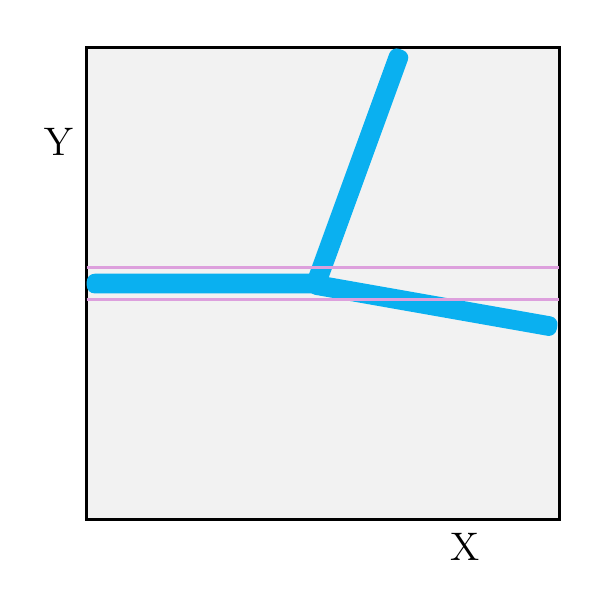
\begin{tikzpicture}
  \pic {actar};

  \pic (beam) {track={0/3/3/0/generic}};
  \pic (light) {track={3/3/6.25/70/generic}};
  \pic (heavy) {track={3-0.2/3/6/-10/generic}};

  % define line coordinates
  \coordinate (up0) at (0, 3.2);
  \coordinate (up1) at (6, 3.2);
  \coordinate (low0) at (0, 2.8);
  \coordinate (low1) at (6, 2.8);
  \draw[very thick, line] (up0) -- (up1);
  \draw[very thick, line] (low0) -- (low1);
\end{tikzpicture}

After applying the breakchi2 operation:

\tikzsetnextfilename{break_chi2_1}
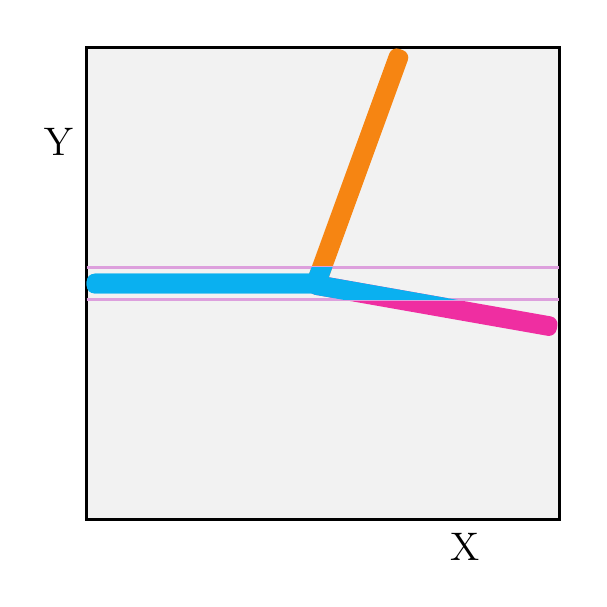
\begin{tikzpicture}
  \pic {actar};

  \pic (beam) {track={0/3/3/0/generic}};
  \pic (light) {track={3/3/6.25/70/light}};
  \pic (heavy) {track={3-0.2/3/6/-10/heavy}};

  % define line coordinates
  \coordinate (up0) at (0, 3.2);
  \coordinate (up1) at (6, 3.2);
  \coordinate (low0) at (0, 2.8);
  \coordinate (low1) at (6, 2.8);
  \draw[very thick, line] (up0) -- (up1);
  \draw[very thick, line] (low0) -- (low1);

  \begin{scope}
    \clip (up0) -- (up1) -- (low1) -- (low0);  % Clip between the lines
    \pic (beam) {track={0/3/3/0/generic}};
    \pic (light) {track={3/3/6.25/70/generic}};
    \pic (heavy) {track={3-0.2/3/6/-10/generic}};
  \end{scope}
\end{tikzpicture}

\end{document}
